\chapter{Baza danych}

\section{Wstęp}
Dane wytwarzane przez system muszą być nieulotne. Z~tego powodu istnieje potrzeba składowania ich na dysku twardym. System zapisuje dane w~relacyjnej bazie danych zgodnej ze standardem SQL. 

\medskip
Wykorzystanym (i~skonfigurowanym) systemem zarządzania relacyjną bazą danych (ang. Relational Database Management System, RDBMS) jest H2 w~trybie wbudowanym (ang. embedded mode). Autor nie widzi potrzeby wykorzystania na potrzeby pracy inżynierskiej bazy danych w~trybie klient-server (ang. client-server mode). Zarówno wykorzystywany system bazy danych, jak i~tryb w~którym jest ona uruchomiana są konfigurowalne poprzez plik \textquote{application.properties}. Jeżeli zaistnieje potrzeba zmiany systemu zarządzania relacyjną bazą danych można to zrobić. Jedynym wymogiem jest, by była to baza relacyjna zgodna ze standardem SQL.

\medskip
Autor projektując bazę danych zastosował podejście \textquote{najpierw kod} (ang. code-first). Oznacza to, że autor zaprojektował bazę danych, jako zbiór encji (ang. entities) - klas języka Java zgodnych ze standardem mapowania relacyjno-obiektowego w~tym języku (tj. Java Persistence API, JPA). Za utworzenie odpowiednich tabel bazodanych, na podstawie istniejących encji, odpowiedzialny jest zastosowany silnik mapowania relacyjno-obiektowego - implementacja JPA - Hibernate. Dla każdej encji wspominany silnik utworzył odpowiadającą jej tabelę w~bazie danych.

\section{Schemat bazy danych}

\medskip
Rysunek \ref{diagram} na stronie \pageref{diagram} przedstawia zastosowany w~systemie schemat bazy danych. Rysunek ten zawiera tabele i~istniejące pomiędzy nimi powiązania. 

\begin{landscape}
\begin{figure}[!ht]
    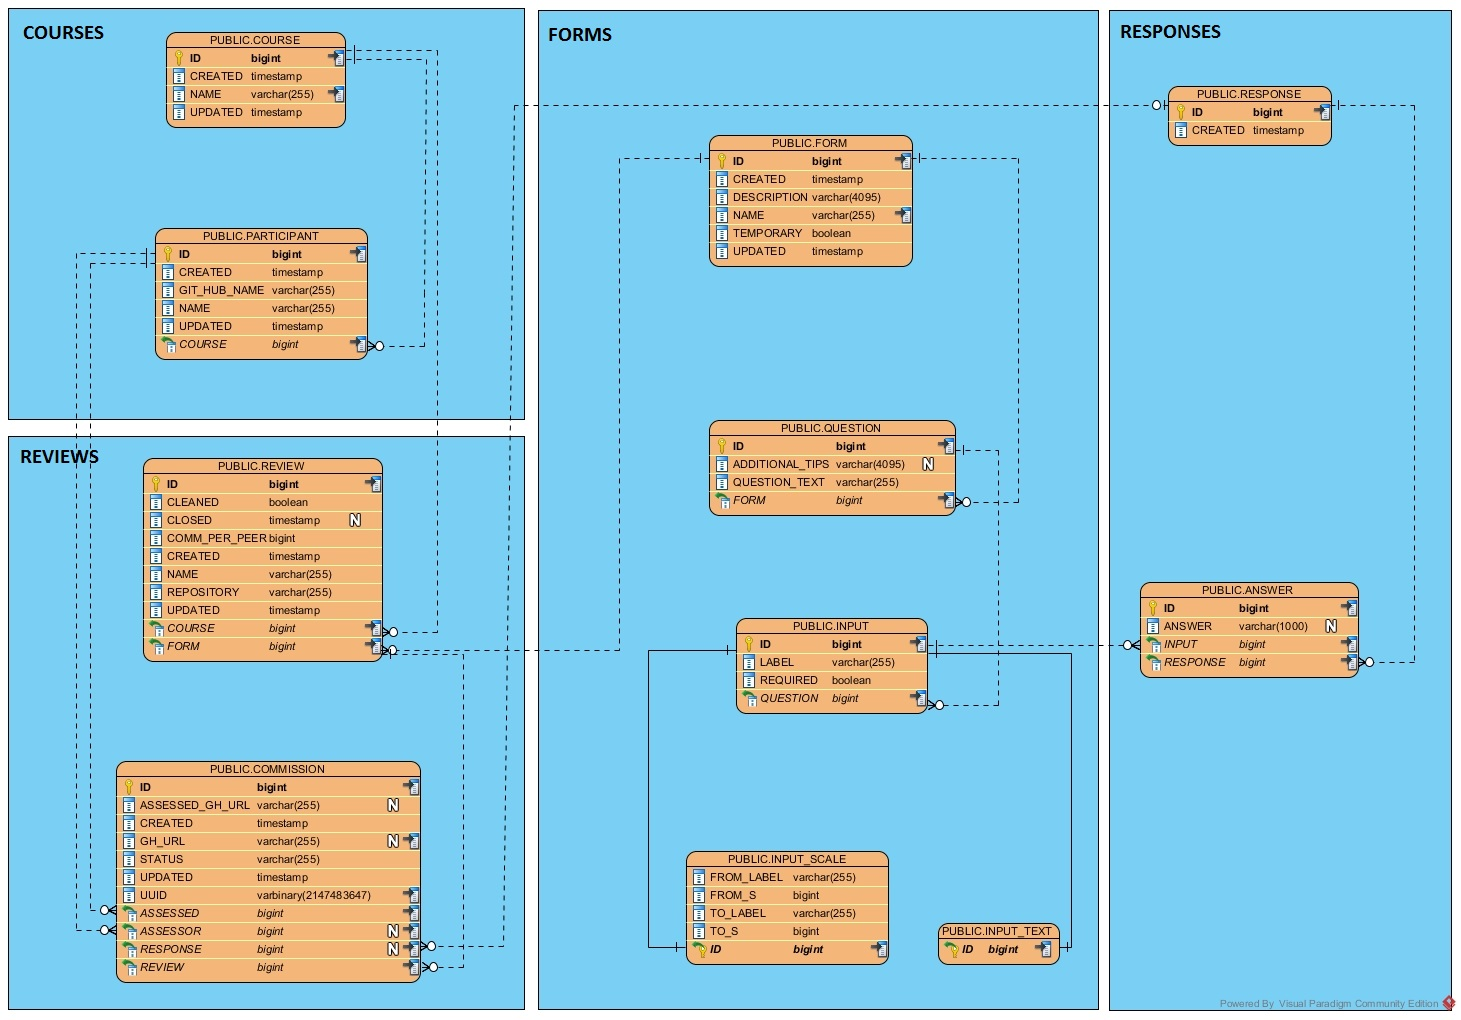
\includegraphics[width=600px]{diagram}
    \caption{Schemat bazy danych}
    \label{diagram}
\end{figure}
\end{landscape}

Autor podzielił model bazy danych na cztery części wzajemnie ze sobą powiązane:
\begin{enumerate}
    \item kursy (ang. courses) - encje odpowiedzialne za kursy i~uczestników;
    \item formularze (ang. forms) - encje odpowiedzialne za system formularzy;
    \item przeglądy (ang. review) - encje odpowiedzialne za przeglądy i~zlecenia;
    \item odpowiedzi (ang. responses) - encje odpowiedzialne za odpowiedzi na zlecenia przeglądów.
\end{enumerate}

\medskip
Cechą wspólną wszystkich encji jest to, że system zapisuje w~atrybutach czas ich utworzenia (\textquote{created}). Większość z~nich zawiera także czas ostatniej aktualizacji (\textquote{updated}). Czas aktualizacji nie jest notowany dla encji, które~z założenia są niemodyfikowalne (ang. immutable)~i nie będą zmieniane.

\subsection{Kursy}
Kursy zostały opisane przy użyciu dwóch encji. Pierwsza z~nich \textquote{course} odpowiada za przechowywanie informacji na temat utworzonych kursów - nadanej nazwy (\textquote{name}),. Druga z~encji to \textquote{participant} i~przechowuje informacje o~uczestnikach zapisanych do danego kursu - imię (\textquote{name}), nazwa konta w~usłudze GitHub (\textquote{githubname}).

\subsection{Formularze}
Każdy formularz posiada odpowiedni wpis w~encji \textquote{form}. Formularz charakteryzuje się nazwą (\textquote{name}). Zawiera także opis (\textquote{description)}, listę pytań (\textquote{question}) i~znacznikiem, czy jest to wpis tymczasowy (\textquote{temporary}). Wpis tymczasowy to atrybut związany z~zastosowaną implementacją podglądu formularza podczas jego tworzenia. Wpis oznaczony przez system jako tymczasowy nie może zostać użyty na innych etapach i~zostanie automatycznie usunięty przy najbliższej okazji.

\medskip
Pytania, które wchodzą w~skład formularza posiadają takie atrybuty jak: treść pytania (\textquote{question\textunderscore text}), opcjonalne informacje dodatkowe (\textquote{additional\textunderscore tips}). Pytanie zawiera także listę kontrolek (\textquote{input}), które mogą być typu skala (\textquote{input\textunderscore scale}) lub tekst (\textquote{input\textunderscore text}).

\subsection{Przeglądy}
Encje związane z~przeglądami to przegląd (\textquote{review}) i~zlecenie (\textquote{commission}). Przegląd jest ogólnym pojęciem i~jest związany z~grupą. Prowadzący zleca przegląd w~grupie. Przegląd może składać się z~wielu zleceń. Zlecenie jest to pojedyncze zadanie ocenienia pracy autorstwa kursanta A~przez innego kursanta B.

\medskip
\clearpage
Przegląd zawiera takie atrybuty jak:
\begin{itemize}
    \item nazwa (\textquote{name});
    \item nazwa źródłowego repozytorium z~ocenianym zadaniem (\textquote{repository});
    \item liczba zleceń w~ramach przeglądu przypadająca na jednego kursanta (\textquote{comm\textunderscore per\textunderscore peer});
    \item znacznik, czy przegląd został już zamknięty (\textquote{closed});
    \item odnośnik do zastosowanego formularza (\textquote{form});
    \item odnośnik do kursu dla którego przegląd został zlecony (\textquote{course}).
\end{itemize}

\medskip
Zlecenie zawiera następujące atrybuty:
\begin{itemize}
    \item odnośnik do przeglądu, do którego zlecenie nalęży (\textquote{review});
    \item odnośnik do kursanta, którego praca jest oceniania (\textquote{assessed});
    \item odnośnik do kursanta, który ma dokonać oceny (\textquote{assessor});
    \item adres URL do repozytorium z~ocenianą pracą (\textquote{assessed\textunderscore gh\textunderscore url});
    \item indywidualny numer przeglądu, zgodny ze standardem UUID4 (\textquote{uuid});
    \item status przeglądu (\textquote{status});
    \item odnośnik do udzielonej odpowiedzi (\textquote{response}).
\end{itemize}

\subsection{Odpowiedzi}
Każde zlecenie zawiera odnośnik do udzielonej odpowiedzi. Za przechowywanie odpowiedzi odpowiadają encje \textquote{response} i~\textquote{answer}. Pierwsza z~nich nie zawiera szczególnych atrybutów - jest to jedynie informacja, że odpowiedź została udzielona. Jedynym atrybutem jest czas udzielenia odpowiedzi (\textquote{created}).

\medskip
Dla każdej kontrolki, która była w~formularzu przypisanym do zlecenia, utworzony zostaje wpis typu \textquote{answer}. Encja taka zawiera odnośnik do kontrolki, której dotyczy (\textquote{input}), odpowiedź udzieloną przez kursanta (\textquote{answer}), oraz odnośnik do encji \textquote{response}, która identyfikuje zlecenie.

% ex: set tabstop=4 shiftwidth=4 softtabstop=4 noexpandtab fileformat=unix filetype=tex spelllang=pl,en spell:
